% !TeX program = pdflatex
% Contando con la torre de derivadas -- el teorema de Budan-Fourier en Lean 4 (ES).
% Espejo de budan-fourier-lean.tex. Mismas figuras (figures/), captions en español.
% Verificado contra la fuente Lean 2026-06-16 (lake env lean BudanFourier.lean, exit 0;
% #print axioms BudanFourier.budan_fourier -> propext, Classical.choice, Quot.sound).

\documentclass[11pt]{article}
\usepackage[T1]{fontenc}
\usepackage[spanish,es-noquoting]{babel}
\usepackage{lmodern}
\usepackage{amsmath,amssymb,amsthm,booktabs,graphicx,hyperref}
\usepackage{xurl}
\usepackage[table]{xcolor}
\definecolor{ggteal}{HTML}{1B6F8C}
\definecolor{ggband}{HTML}{DCE7EB}
\definecolor{ggamber}{HTML}{E08A1E}
\definecolor{ggplum}{HTML}{7B4B94}
\usepackage[margin=1in]{geometry}
\usepackage{microtype}
\usepackage{float}
\usepackage[most]{tcolorbox}
\usepackage{tikz}
\usetikzlibrary{arrows.meta,positioning}
\graphicspath{{figures/}}
\setlength{\emergencystretch}{2em}
\newtheorem{theorem}{Teorema}
\newtheorem{lemma}{Lema}
\newtheorem{proposition}{Proposici\'on}
\newtheorem{remark}{Observaci\'on}
\newcommand{\lean}[1]{\texttt{#1}}
\newcommand{\R}{\mathbb{R}}
\newcommand{\V}{\mathrm{V}}
\hypersetup{colorlinks=true,linkcolor=ggteal,citecolor=ggteal,urlcolor=ggteal}
\newtcbox{\keybox}{on line,boxrule=0.9pt,colframe=ggteal,colback=ggband!40,
  arc=3pt,left=8pt,right=8pt,top=5pt,bottom=5pt}
\newcommand{\keyeq}[1]{\begin{center}\keybox{$\displaystyle #1$}\end{center}}
\newtcolorbox{recipebox}[1]{colframe=ggamber,colback=ggamber!8,arc=3pt,boxrule=0.8pt,
  title=\textbf{#1},coltitle=white,colbacktitle=ggamber}

\title{\bf Contando con la torre de derivadas\\[4pt]
  \large\normalfont El teorema de Budan--Fourier, verificado por m\'aquina en Lean~4}
\author{Carles Mar\'in\thanks{Formalizado con la asistencia de un sistema de IA (Claude,
Anthropic); la matem\'atica es cl\'asica, y toda afirmaci\'on, alcance y limitaci\'on es
responsabilidad del autor. La frontera de la contribuci\'on se expone sin adornos en la
Secci\'on~\ref{sec:boundary}, y es el n\'ucleo de Lean---no el asistente---quien certifica las
demostraciones.}\\[3pt]
  \normalsize Investigador independiente\\
  \normalsize \texttt{karlesmarin@gmail.com}}
\date{Junio de 2026}

\begin{document}
\maketitle

\begin{abstract}
Presento una formalizaci\'on completa y \lean{sorry}-free en Lean~4, sobre Mathlib, del
\emph{teorema de Budan--Fourier}: para un polinomio real no nulo $p$ y un intervalo $(a,b]$ cuyos
extremos no son ra\'ices, el n\'umero de ra\'ices reales de $p$ en $(a,b]$, \emph{contadas con
multiplicidad}, es a lo sumo la ca\'ida $\V(a)-\V(b)$ en las variaciones de signo de la torre de
derivadas $p,\,p',\,p'',\dots,p^{(\deg p)}$, y difiere de ella en un n\'umero par:
\[
  \#\mathrm{ra\acute{\imath}ces}(a,b]\ \le\ \V(a)-\V(b),\qquad
  \V(a)-\V(b)-\#\mathrm{ra\acute{\imath}ces}(a,b]\ \text{es par.}
\]
No se localiza ninguna ra\'iz; se leen y se restan signos a lo largo de una torre de derivadas. La
matem\'atica es cl\'asica y se ha formalizado una vez antes, en Isabelle/HOL por Wenda Li~\cite{liBF};
hasta donde s\'e---a partir de b\'usquedas en Loogle y Mathlib en junio de 2026
(Secci\'on~\ref{sec:boundary})---esta es la primera demostraci\'on del teorema de Budan--Fourier en
Lean. Mathlib incluye la regla de los signos de Descartes (\lean{Polynomial.signVariations}, el
recuento de coeficientes) pero ni la torre de derivadas ni el teorema en un intervalo; este trabajo
llena ese hueco y es el compa\~nero exacto de una formalizaci\'on reciente del teorema de Sturm en
Lean~\cite{sturmlean}, con la que comparte el instrumental de variaci\'on de signo. La contribuci\'on
es la formalizaci\'on y la maquinaria reutilizable que la demostraci\'on exigi\'o: dos
\emph{ladrillos de monoton\'ia} de un solo paso que fijan el signo de una derivada justo fuera de una
ra\'iz, un par abstracto de operaciones sobre listas (\lean{Rseq}/\lean{Lseq}) que desacopla la
contabilidad de signos de los polinomios, y la identificaci\'on de la racha inicial de ceros de la
torre con la multiplicidad de la ra\'iz. El teorema principal \lean{budan\_fourier} depende solo de
los tres axiomas est\'andar \lean{propext}, \lean{Classical.choice}, \lean{Quot.sound}.
\end{abstract}

\medskip
\noindent\emph{Lo que encontrar\'as aqu\'i.} Es una visita guiada breve, no un manual, y est\'a
construida como un collar de cuentas: cada secci\'on termina entregando al lector la pregunta que
responde la siguiente. La primera pregunta c\'omo una diferencia de dos enteros puede acotar---y casi
contar---las ra\'ices (Secci\'on~\ref{sec:q1}); la segunda, por qu\'e el recuento se mueve solo en los
puntos cr\'iticos, y all\'i por la \emph{multiplicidad}, salvo un excedente par
(Secci\'on~\ref{sec:q2}); la tercera, d\'onde la demostraci\'on se resiste de verdad a formalizarse,
ahora que la torre ya no es una cadena coprima (Secci\'on~\ref{sec:q3}); la cuarta, qu\'e queda gratis
una vez certificado el teorema---incluido por qu\'e la regla de Descartes sobrecuenta por un n\'umero
par (Secci\'on~\ref{sec:q4}). Los lemas que soportan el peso se re\'unen en una tabla
(Secci\'on~\ref{sec:blocks}); los l\'imites honestos se enuncian sin barniz en la
Secci\'on~\ref{sec:boundary}; y la secci\'on final plantea, a modo de reflexi\'on, las preguntas que
prefiero llevarme al pr\'oximo paper antes que fingir haber resuelto. Si solo lees dos cosas, lee el
Teorema~\ref{thm:bf} y la Figura~\ref{fig:tower}; el resto es el argumento que los conecta.

\begin{figure}[htbp]
\centering
\begin{tikzpicture}[
  obj/.style={draw=ggteal,thick,rounded corners=2pt,fill=ggband!40,align=center,
    font=\small,inner sep=4pt,minimum height=11mm,text width=24mm},
  q/.style={font=\scriptsize\itshape,text=ggamber!80!black,align=center,fill=white,inner sep=1pt},
  arr/.style={-{Stealth[length=2.4mm]},thick,ggteal}]
  \node[obj] (seq) {una torre de\\derivadas};
  \node[obj,right=33mm of seq] (count) {un recuento de\\cambios de signo};
  \node[obj,right=33mm of count] (quantum) {una ra\'iz,\\un paso / mult.};
  \node[obj,below=16mm of quantum] (glue) {pegar los pasos\\sobre $(a,b]$};
  \node[obj,left=33mm of glue] (free) {Descartes\\y su hueco par};
  \node[obj,left=33mm of free,fill=ggamber!25,draw=ggamber] (done)
    {\textbf{Budan--}\\\textbf{Fourier,}\\\textbf{verificado}};
  \draw[arr] (seq) -- node[q,above=2pt] {P1:\\¿contar?} (count);
  \draw[arr] (count) -- node[q,above=2pt] {P2: ¿en\\cu\'anto?} (quantum);
  \draw[arr] (quantum) -- node[q,right=2pt,fill=none] {P3: ¿se\\resiste?} (glue);
  \draw[arr] (glue) -- node[q,above=2pt] {P4: ¿qu\'e\\queda gratis?} (free);
  \draw[arr] (free) -- (done);
\end{tikzpicture}
\caption{El mapa del lector. De la torre de derivadas a un recuento certificado en un intervalo y lo
que rinde aguas abajo; cada flecha es la pregunta que su secci\'on responde. Cada nodo es un bloque de
Lean \lean{sorry}-free.}
\label{fig:readermap}
\end{figure}

\section{La pregunta que lo inicia todo}\label{sec:intro}

¿Cu\'antas ra\'ices reales tiene un polinomio entre aqu\'i y all\'i---y se puede decir sin encontrar
ni una sola de ellas? La regla de los signos de Descartes (1637)~\cite{descartes} lee una \emph{cota}
de las ra\'ices positivas a partir de los signos de los coeficientes. A principios del siglo XIX
Fran\c{c}ois Budan~\cite{budan} y Joseph Fourier~\cite{fourier} la afinaron de la semirrecta a un
intervalo arbitrario, y de los coeficientes a la \emph{torre de derivadas}: al\'inea
\[
  p,\ p',\ p'',\ \dots,\ p^{(\deg p)},
\]
lee el n\'umero $\V(x)$ de cambios de signo de esta lista en un punto $x$ (descartando ceros), y la
ca\'ida $\V(a)-\V(b)$ a lo largo de $(a,b]$ es una cota superior del n\'umero de ra\'ices all\'i.
Sturm~\cite{sturm} cerr\'o m\'as tarde la brecha entre cota y recuento, pero con una sucesi\'on
\emph{distinta}---los restos eucl\'ideos negados---y solo para ra\'ices distintas; el enunciado de
Budan--Fourier, sobre la torre y con multiplicidad, conserv\'o dos rasgos que el de Sturm no: cuenta
cada ra\'iz tantas veces como su orden, y su cota difiere del recuento verdadero en un n\'umero
\emph{par}. Ese hueco par no es ruido. Es la huella de las ra\'ices complejas que el intervalo no
puede ver, y es la raz\'on por la que la regla de Descartes, la sombra de este teorema cuando
$b\to\infty$, sobrecuenta por una cantidad par y nunca impar.

El teorema es cl\'asico y se ha verificado por m\'aquina una vez, en Isabelle/HOL, por Wenda
Li~\cite{liBF}, quien adem\'as lo us\'o para impulsar un procedimiento certificado de recuento de
ra\'ices y, de paso, extendi\'o el teorema de Sturm a la multiplicidad. Lo que no se hab\'ia hecho es
verificarlo en \emph{Lean}. Mathlib incluye la regla de Descartes---la funci\'on
\lean{Polynomial.signVariations}, el recuento de coeficientes---pero no la sucesi\'on de la torre de
derivadas ni el teorema en un intervalo. Este paper llena ese hueco. Es, para ser exacto, un
primero-en-Lean y no un primero-en-cualquier-sistema;\footnote{Reivindicaci\'on de prioridad basada en
b\'usquedas de Loogle y un \lean{grep} de Mathlib en junio de 2026; la formalizaci\'on previa en
Isabelle/HOL se acredita en la Secci\'on~\ref{sec:boundary}.} el valor est\'a en a\~nadir el
compa\~nero natural del teorema de Sturm a una biblioteca que carec\'ia de \'el, y en las piezas
reutilizables que la demostraci\'on deja tras de s\'i.

Llegu\'e a \'el igual que a Sturm~\cite{sturmlean}: preguntando qu\'e resultados cl\'asicos del
recuento de ra\'ices reales le siguen faltando a una biblioteca madura. Con el teorema de Sturm ya
hecho y su instrumental de variaci\'on de signo ya escrito, Budan--Fourier era la siguiente ausencia
conspicua---y, result\'o, aquella cuyo an\'alisis local es genuinamente \emph{m\'as dif\'icil} que el
de Sturm, por una raz\'on que merece el viaje. El resto del paper es ese viaje, contado como las
cuatro preguntas que un lector atento hace por turno.

\section{P1: ¿c\'omo puede una diferencia de signos acotar, y casi contar, las ra\'ices?}\label{sec:q1}

\emph{Cuenta hist\'orica.} La torre, el recuento en un intervalo y el refinamiento de paridad son de
Budan y Fourier~(\cite{budan,fourier}; la exposici\'on moderna de libro de texto es
Basu--Pollack--Roy~\cite{bpr}, Cap.~2, y Akritas~\cite{akritas} desenreda el registro hist\'orico).
Nada en esta secci\'on es matem\'atica nueva; el Lean est\'a en \lean{BudanFourier.lean}, las
definiciones \lean{fourierSeq} y \lean{fourierVar}.

Precisemos los dos ingredientes. La \emph{sucesi\'on de Fourier} de $p$ es su torre de derivadas,
\[
  \lean{fourierSeq}\,p\ =\ \big[\,p,\ p',\ p'',\ \dots,\ p^{(\deg p)}\,\big],
\]
una \lean{List} de polinomios de longitud $\deg p + 1$. El recuento es
\[
  \V_p(x)\ =\ \lean{fourierVar}\,p\,x,
\]
el n\'umero de cambios de signo en la lista de signos evaluados tras eliminar los ceros. Un solo
\lean{rfl} registra que esta es la misma construcci\'on que el desarrollo de Sturm ya analiz\'o,
aplicada a una lista distinta: \lean{fourierVar p x = Sturm.signVarAt (fourierSeq p) x}. Esa l\'inea
deja que todo el instrumental del paper de Sturm---constancia local en un intervalo sin ra\'ices, el
recuento recursivo \lean{signChanges}, la recursi\'on del par cabecero---act\'ue tal cual sobre la
torre.

No volver\'e a derivar ese instrumental aqu\'i; es el tema del paper compa\~nero~\cite{sturmlean}. Los
dos son deliberadamente papers \emph{distintos}, y conviene decir con claridad por qu\'e. El teorema
de Sturm corre sobre la cadena de restos negados, cuenta ra\'ices \emph{distintas} y es una igualdad
exacta cuyo an\'alisis local toca solo un par de la cadena. El teorema de Budan--Fourier de aqu\'i
corre sobre la \emph{torre de derivadas}, cuenta ra\'ices \emph{con multiplicidad}, es una
\emph{desigualdad} con un refinamiento de paridad par, y---porque la torre no es una cadena
coprima---su an\'alisis local debe tratar un \emph{bloque que se anula} entero de una vez.
\textbf{El mismo instrumental debajo, un teorema genuinamente distinto encima:} este paper importa la
maquinaria compartida por cita y gasta sus p\'aginas solo en lo que la torre fuerza y la cadena no.

\begin{theorem}[Budan--Fourier, en Lean~4; \lean{budan\_fourier}]\label{thm:bf}
Sea $p$ un polinomio real no nulo y $a<b$ con $p(a)\ne0$ y $p(b)\ne0$. Entonces, escribiendo
$\#\mathrm{ra\acute{\imath}ces}(a,b]$ por el n\'umero de ra\'ices reales de $p$ en $(a,b]$ contadas con
multiplicidad,
\keyeq{\#\mathrm{ra\acute{\imath}ces}(a,b]\ \le\ \V_p(a)-\V_p(b)\quad\text{y}\quad
  \V_p(a)-\V_p(b)-\#\mathrm{ra\acute{\imath}ces}(a,b]\ \text{es par.}}
El enunciado es \lean{sorry}-free; \lean{\#print axioms BudanFourier.budan\_fourier} reporta solo
\lean{propext}, \lean{Classical.choice}, \lean{Quot.sound}.
\end{theorem}

Que una diferencia de dos enteros controle un recuento de ra\'ices es, a primera vista, un peque\~no
milagro, as\'i que vale la pena verlo ocurrir a mano---y ver sus dos caras, la multiplicidad y el
hueco par, en un ejemplo cada una.

\emph{Un caso comprobable a mano: la multiplicidad.} Toma $p_A(x)=(x-1)^2(x+1)=x^3-x^2-x+1$, con una
ra\'iz simple en $-1$ y una ra\'iz doble en $1$. La torre es
\[
  p_A,\quad p_A'=3x^2-2x-1,\quad p_A''=6x-2,\quad p_A'''=6,
\]
y leyendo los signos en los extremos de $(-2,2]$ se obtiene $\V(-2)=3$ y $\V(2)=0$, de modo que
$\V(-2)-\V(2)=3$, exactamente el recuento de ra\'ices \emph{con multiplicidad} ($1$ en $x=-1$, $2$ en
$x=1$). La escalera de $\V$ (Figura~\ref{fig:tower}(A)) cae en uno en la ra\'iz simple y en \emph{dos}
en la ra\'iz doble: \textbf{la altura del escal\'on es la multiplicidad de la ra\'iz}. Aqu\'i la
desigualdad del Teorema~\ref{thm:bf} es una igualdad. La Tabla~\ref{tab:signsA} lee el ejemplo punto
por punto; cada entrada se reverifica en aritm\'etica exacta por el script de la figura.

\emph{Un caso comprobable a mano: el excedente par.} Toma $p_B(x)=x^2+1$, sin ra\'iz real alguna. Su
torre es $p_B,\ 2x,\ 2$, y $\V(-2)=2$ mientras $\V(2)=0$, de modo que la cota es $\V(-2)-\V(2)=2$ y el
recuento verdadero es $0$. \textbf{El excedente es $2$---par.} Mirando m\'as de cerca
(Figura~\ref{fig:tower}(B)), la escalera cae en $x=0$, que es un cero del miembro \emph{interior}
$p_B'=2x$ pero no una ra\'iz de $p_B$: la ca\'ida ocurre en un punto cr\'itico que ninguna ra\'iz de
$p_B$ explica, y es necesariamente \emph{par} (aqu\'i $\V(a)=\V(b)+0+2e$ con $e=1$)---el rastro local
del par conjugado $\pm i$ que el intervalo real no puede ver. Este es el fen\'omeno que la regla de
Descartes exhibe globalmente; Budan--Fourier lo localiza.

\begin{figure}[htbp]
\centering
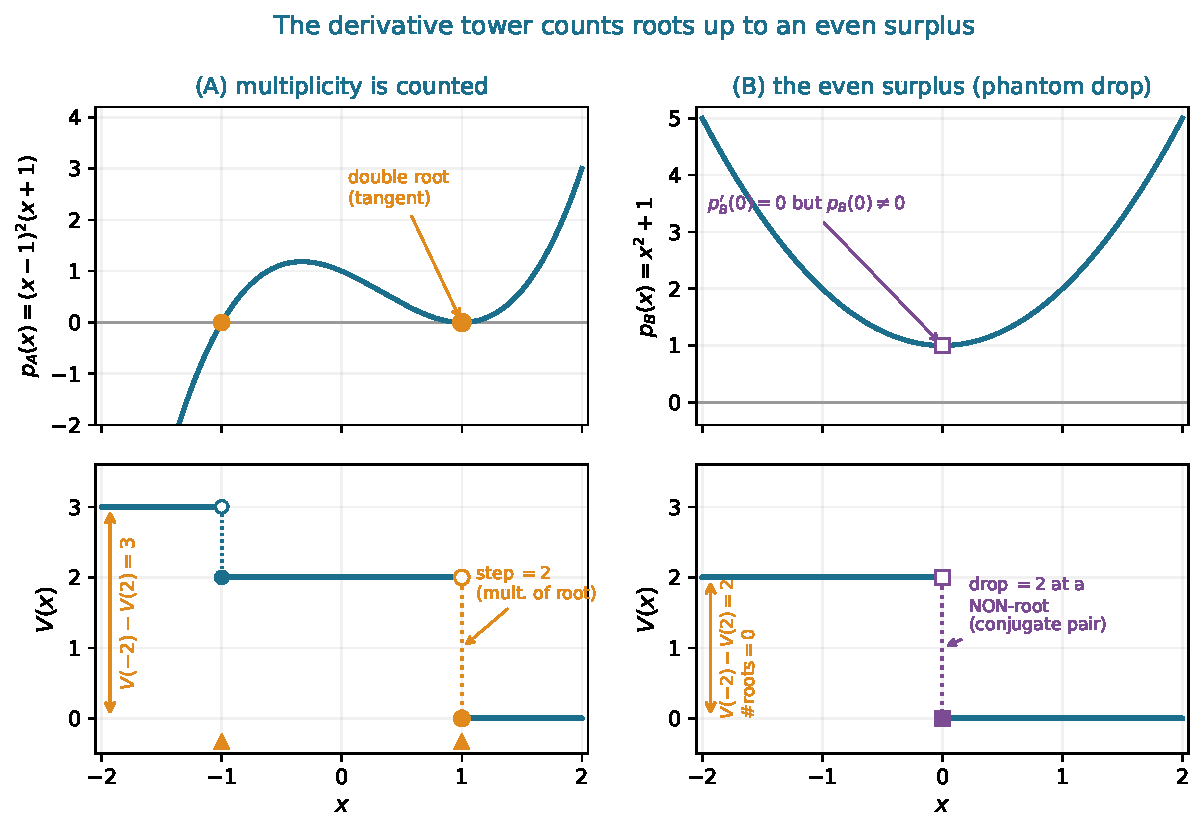
\includegraphics[width=\textwidth]{budan_fig1_tower}
\caption{La torre de derivadas cuenta ra\'ices salvo un excedente par. \emph{(A)}
$p_A=(x-1)^2(x+1)$: $\V$ cae en $1$ en la ra\'iz simple $x=-1$ y en $2$ en la ra\'iz doble $x=1$
(c\'irculo abierto = el valor justo a la izquierda, relleno = el valor en el punto, en el escal\'on
inferior). El descenso sobre $(-2,2]$ es el recuento de ra\'ices \emph{con multiplicidad}, as\'i que
la desigualdad es ajustada. \emph{(B)} $p_B=x^2+1$, sin ra\'iz real: $\V$ cae igualmente en $2$, en
$x=0$, donde el miembro interior $p_B'$ se anula pero $p_B$ no---el excedente par, la firma de un par
conjugado. Cada signo y recuento dibujado se afirma contra aritm\'etica exacta antes de dibujar.}
\label{fig:tower}
\end{figure}

\begin{table}[htbp]
\centering\small
\rowcolors{2}{ggband!35}{white}
\begin{tabular}{@{}rccccr@{}}
\toprule
\rowcolor{ggteal!18}
$x$ & $p_A$ & $p_A'$ & $p_A''$ & $p_A'''$ & $\V(x)$ \\
    & {\scriptsize$x^3{-}x^2{-}x{+}1$} & {\scriptsize$3x^2{-}2x{-}1$} & {\scriptsize$6x{-}2$} & {\scriptsize$6$} & \\
\midrule
$-2$            & $-$ & $+$ & $-$ & $+$ & $3$ \\
$-\tfrac32$     & $-$ & $+$ & $-$ & $+$ & $3$ \\
$-1$ {\scriptsize(ra\'iz)}        & $0$ & $+$ & $-$ & $+$ & $2$ \\
$0$             & $+$ & $-$ & $-$ & $+$ & $2$ \\
$\tfrac12$      & $+$ & $-$ & $+$ & $+$ & $2$ \\
$1$ {\scriptsize(ra\'iz doble)}  & $0$ & $0$ & $+$ & $+$ & $0$ \\
$2$             & $+$ & $+$ & $+$ & $+$ & $0$ \\
\bottomrule
\end{tabular}
\caption{El Ejemplo A le\'ido sobre la torre. $\V$ cae en $1$ en la ra\'iz simple $x=-1$ y en $2$ en
la ra\'iz doble $x=1$: la ca\'ida cuenta multiplicidad. En $(-2,2]$, $\V(-2)-\V(2)=3$ es el recuento
de ra\'ices con multiplicidad, as\'i que aqu\'i la desigualdad de Budan--Fourier es ajustada. La tabla
entera se regenera y se comprueba en aritm\'etica exacta por \lean{budan\_fig1\_tower.py}.}
\label{tab:signsA}
\end{table}

La imagen tras las tablas es la escalera que da nombre al m\'etodo del paper. Dibuja $\V(x)$ mientras
$x$ barre la recta: es plana casi en todas partes y cae solo en los \emph{puntos cr\'iticos}---puntos
donde alg\'un miembro de la torre se anula. En una ra\'iz de $p$ cae por la multiplicidad; en un punto
cr\'itico que no es ra\'iz de $p$ a\'un puede caer, por una cantidad par. Todo el contenido de las dos
secciones siguientes est\'a en demostrar que la escalera tiene exactamente esta forma. Esa es la
cuenta que esta secci\'on entrega: \emph{¿por qu\'e se mueve $\V$ solo en los puntos cr\'iticos, y
all\'i exactamente por la multiplicidad m\'as un n\'umero par?}

\section{P2: ¿por qu\'e se mueve el recuento solo en los puntos cr\'iticos, y en cu\'anto?}\label{sec:q2}

\emph{Cuenta hist\'orica.} El an\'alisis local es el coraz\'on de toda demostraci\'on de
Budan--Fourier. Lo que lo hace m\'as dif\'icil que el de Sturm es estructural: la cadena de Sturm est\'a
construida para que miembros consecutivos sean coprimos, de modo que no se anulan dos a la vez y el
an\'alisis en una ra\'iz toca solo el par cabecero $(p,p')$. La torre de derivadas no tiene esa
suerte---$p$ y $p'$ \emph{s\'i} se anulan juntos en una ra\'iz m\'ultiple, y un \emph{bloque} entero de
miembros consecutivos $p^{(i)},\dots,p^{(j)}$ puede anularse en un punto. El Lean est\'a en los lemas
\lean{sign\_eval\_right\_vanish}, \lean{sign\_eval\_left\_vanish} (los dos ladrillos) y
\lean{fourierVar\_drop\_at\_critical\_point} (su ensamblaje).

Lejos de los puntos cr\'iticos cada miembro conserva su signo---un polinomio no puede cambiar de signo
sin una ra\'iz, por el teorema del valor intermedio---as\'i que $\V$ es localmente constante
(\lean{fourierVar\_eq\_of\_no\_root}, heredado tal cual del instrumental de Sturm). Por eso la escalera
es plana entre cr\'iticos. Toda la acci\'on est\'a en un punto cr\'itico $c$, y la dificultad nueva es
el bloque que se anula.

\emph{Los dos ladrillos.} La torre tiene un rasgo que reemplaza a la coprimalidad: cada miembro es la
derivada del anterior, $p^{(k+1)}=(p^{(k)})'$. As\'i que si $p^{(k)}(c)=0$ mientras $p^{(k+1)}$
mantiene un signo $s$ no nulo constante justo fuera de $c$, entonces $p^{(k)}$ es estrictamente
mon\'otono all\'i, y su signo justo fuera de $c$ queda forzado---\emph{el mismo} que su derivada
$p^{(k+1)}$ a la derecha, el \emph{opuesto} a la izquierda. Sin desarrollo de Taylor, sin contabilidad
de multiplicidades: una aplicaci\'on del teorema del valor medio.
\begin{recipebox}{Los dos ladrillos de monoton\'ia (receta)}
Si $q(c)=0$ y $q'$ mantiene el signo $s$ no nulo constante en $(c,z]$, entonces
$\mathrm{sign}\,q(z)=s$ (\lean{sign\_eval\_right\_vanish}). Si en cambio $q'$ mantiene el signo $s$ en
$[z,c)$, entonces $\mathrm{sign}\,q(z)=-s$ (\lean{sign\_eval\_left\_vanish}). Aplica esto subiendo un
bloque que se anula, anclado en su primer miembro \emph{no} nulo (la derivada de mayor orden justo
pasado el bloque): \textbf{a la derecha de $c$ cada miembro que se anula copia el signo de su
derivada}, as\'i que el bloque colapsa a un solo signo y no aporta \emph{ning\'un} cambio de signo;
\textbf{a la izquierda cada uno toma el opuesto del signo de su derivada}, as\'i que el bloque
\emph{alterna} y aporta un cambio de signo por miembro.
\end{recipebox}

\begin{figure}[htbp]
\centering
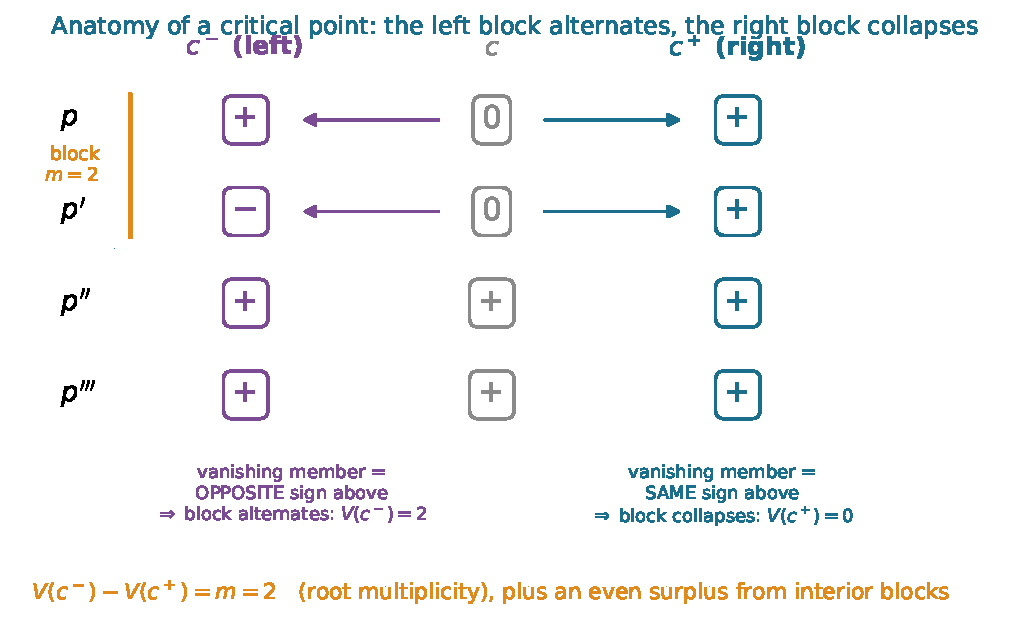
\includegraphics[width=0.74\textwidth]{budan_fig2_critical}
\caption{Anatom\'ia de un punto cr\'itico, para la ra\'iz doble $c=1$ de $p_A$ (el bloque $p,p'$ se
anula, $m=2$). Leyendo cada signo justo fuera de $c$ desde la derivada de ese miembro: a la derecha
(turquesa) un miembro que se anula copia el signo de su derivada---el bloque colapsa, $\V(c^+)=0$; a
la izquierda (ciruela) toma el opuesto---el bloque alterna, $\V(c^-)=2$. As\'i $\V(c^-)-\V(c^+)=m$, la
multiplicidad, m\'as una cantidad par de cualquier bloque interior. Los signos son exactos de la torre
de $p_A$.}
\label{fig:critical}
\end{figure}

Contar las consecuencias da la ca\'ida local. Justo a la derecha de $c$ la lista de signos de la torre
es la lista en $c$ con cada entrada que se anula reemplazada por el signo de su primer sucesor no
nulo---una operaci\'on sobre listas de signos puras que llamo \lean{Rseq}; justo a la izquierda es lo
mismo con signos \emph{alternados}, \lean{Lseq}. La lista derecha tiene el \emph{mismo} n\'umero de
cambios de signo que la lista en $c$ (\lean{Rseq\_spec}: $\V(c^+)=\V(c)$, el lado derecho no lleva
informaci\'on); la lista izquierda tiene esos \emph{m\'as} la longitud de la racha inicial de ceros
\emph{m\'as} un excedente par de los bloques interiores (\lean{Lseq\_spec}). Escribiendo $m$ por la
racha inicial y empaquetando el excedente como $2e$,
\keyeq{\V(c^-)\ =\ \V(c^+)\ +\ m\ +\ 2e .}
La Figura~\ref{fig:critical} muestra el mecanismo en la ra\'iz doble de $p_A$, donde el bloque $p,p'$
da $\V(1^-)-\V(1^+)=2$. El \'ultimo paso es reconocer $m$: la racha inicial de miembros que se anulan
en $c$ tiene longitud exactamente la \emph{multiplicidad} de $p$ en $c$, porque en caracter\'istica
cero el orden de la primera derivada no nula \emph{es} la multiplicidad. Mathlib lo sabe
(\lean{lt\_rootMultiplicity\_iff\_isRoot\_iterate\_derivative}), y las ra\'ices de $p$ en $(a,b]$ que
caen en $c$ son exactamente esa multiplicidad (\lean{count\_roots}). As\'i $m=\#\mathrm{ra\acute{\imath}ces}(a,b]$
en una ra\'iz genuina, y $m=0$ en un punto cr\'itico que no es ra\'iz---en cuyo caso toda la ca\'ida es
el excedente par, exactamente el Ejemplo B. La forma aditiva $\V(a)=\V(b)+\#\mathrm{ra\acute{\imath}ces}+2e$
empaqueta la desigualdad y la paridad en un solo enunciado que sumar\'a limpiamente a lo largo del
intervalo.

La cuenta que esto entrega es la que m\'as le importa a la m\'aquina: \emph{toda esta imagen es una
frase sobre el papel---``el bloque izquierdo alterna y el derecho colapsa''---pero ¿d\'onde, hecha
formal, se resiste?}

\section{P3: ¿d\'onde se resiste la demostraci\'on a hacerse formal?}\label{sec:q3}

\emph{Cuenta hist\'orica.} Sobre el papel el an\'alisis de bloque es una imagen; hecho formal, es el
\'unico paso genuinamente estructural, porque la alternancia y el colapso deben realizarse \emph{a lo
largo de una lista cuya forma es recursiva}, y las hip\'otesis que justifican cada paso---qu\'e miembro
se anula, qu\'e signo tiene su vecino---est\'an entretejidas con la estructura misma de la torre. El
dispositivo que lo resuelve, el par \lean{Rseq}/\lean{Lseq} junto con sus especificaciones, es la parte
de este desarrollo con menos antecedente directo en los libros: no un teorema nuevo, sino la
ingenier\'ia de demostraci\'on que mantiene honesta la contabilidad. Es el an\'alogo, para la torre, de
la relaci\'on \lean{FlankReduce} que hizo el mismo trabajo para Sturm~\cite{sturmlean}.

La dificultad es precisa. Para comparar $\V(a)$ con $\V(b)$ a trav\'es de $c$, hay que realizar el
colapso-a-la-derecha y la alternancia-a-la-izquierda sobre las listas de signos evaluados, y la regla
de cada entrada depende de si \emph{ese} miembro se anula en $c$ y del signo de su derivada. La
combinatoria de reescribir una lista y el \'algebra de por qu\'e cada reescritura es l\'icita est\'an
entrelazadas, y una demostraci\'on honesta las separa.

La separaci\'on son dos operaciones sobre listas de signos puras, definidas por recursi\'on y probadas
correctas sin mencionar jam\'as un polinomio.
\begin{recipebox}{El desacoplamiento (receta)}
En una lista $s$ de signos (entrada $0$ = miembro que se anula, $\pm1$ = miembro conservado),
\lean{Rseq} reemplaza cada $0$ por el siguiente valor superviviente y \lean{Lseq} lo reemplaza por la
negaci\'on de ese valor. Dos hechos reparten entonces el trabajo. \emph{Combinatorio:} \lean{Rseq\_spec}
muestra que la lista derecha tiene el mismo recuento de cambios de signo que $s$, y \lean{Lseq\_spec}
muestra que la lista izquierda tiene ese recuento m\'as la racha inicial de ceros m\'as un n\'umero
par---esto es inducci\'on pura sobre listas cargando un invariante de paridad del signo cabecero, sin
polinomios. \emph{Estructural:} \lean{signs\_right\_eq\_Rseq} y \lean{signs\_left\_eq\_Lseq} muestran
que la lista de signos evaluados de la torre en $b$ (resp.\ $a$) \emph{es} \lean{Rseq} (resp.\
\lean{Lseq}) de la lista en $c$---esto es la inducci\'on sobre la torre, alimentada por los dos
ladrillos de monoton\'ia y por nada m\'as.
\end{recipebox}

\begin{figure}[htbp]
\centering
\begin{tikzpicture}[
  s/.style={draw=ggteal,rounded corners=1.5pt,minimum size=7.5mm,inner sep=2pt,font=\small,fill=white},
  sz/.style={draw=ggteal,rounded corners=1.5pt,minimum size=7.5mm,inner sep=2pt,font=\small,
    fill=ggband!60,text=gray},
  sl/.style={draw=ggplum,rounded corners=1.5pt,minimum size=7.5mm,inner sep=2pt,font=\small,
    fill=ggplum!10,text=ggplum!80!black},
  sr/.style={draw=ggteal,rounded corners=1.5pt,minimum size=7.5mm,inner sep=2pt,font=\small,
    fill=ggteal!12},
  arr/.style={-{Stealth[length=2.4mm]},thick},
  lbl/.style={font=\scriptsize\itshape,align=center}]
  \node[font=\bfseries\small,text=gray] at (-2.55,0) {en $c$:};
  \node[sz] (c0) at (0,0) {$0$};
  \node[sz] (c1) at (0.85,0) {$0$};
  \node[s]  (c2) at (1.70,0) {$+$};
  \node[s]  (c3) at (2.55,0) {$+$};
  \node[font=\bfseries\small,text=ggplum] at (-2.55,1.5) {$\lean{Lseq}$ (izq., $a$):};
  \node[sl] at (0,1.5) {$+$};
  \node[sl] at (0.85,1.5) {$-$};
  \node[sl] at (1.70,1.5) {$+$};
  \node[sl] at (2.55,1.5) {$+$};
  \node[font=\bfseries\small,text=ggteal] at (-2.55,-1.5) {$\lean{Rseq}$ (der., $b$):};
  \node[sr] at (0,-1.5) {$+$};
  \node[sr] at (0.85,-1.5) {$+$};
  \node[sr] at (1.70,-1.5) {$+$};
  \node[sr] at (2.55,-1.5) {$+$};
  \draw[arr,ggplum] (1.0,0.45) -- (0.4,1.05);
  \draw[arr,ggteal] (1.0,-0.45) -- (0.4,-1.05);
  \node[lbl,text=ggplum!80!black,text width=4.6cm] at (5.6,1.5)
    {un anulado toma el siguiente signo \emph{negado} $\Rightarrow$ el bloque alterna,
     $+1$ por anulado: $\V(c^-)=\V(c)+m+2e$};
  \node[lbl,text=ggteal!80!black,text width=4.6cm] at (5.6,-1.5)
    {un anulado \emph{copia} el siguiente signo $\Rightarrow$ el bloque colapsa, sin cambio nuevo:
     $\V(c^+)=\V(c)$};
  \node[lbl,text=gray,text width=4.6cm] at (5.6,0)
    {una lista de signos pura; \textbf{no aparece ning\'un polinomio}};
\end{tikzpicture}
\caption{El desacoplamiento de la Secci\'on~\ref{sec:q3}, a nivel de listas de signos puras (aqu\'i el
bloque $0,0$ de la ra\'iz doble de $p_A$). \lean{Rseq} y \lean{Lseq} son operaciones sobre listas
puras---una entrada que se anula copia, resp.\ niega, el siguiente signo superviviente---y sus
especificaciones de recuento (\lean{Rseq\_spec}, \lean{Lseq\_spec}) se prueban por inducci\'on sobre
listas sin polinomio a la vista. Los lemas estructurales \lean{signs\_right\_eq\_Rseq}/\lean{signs\_left\_eq\_Lseq}
son el \'unico puente de vuelta a la torre, y se alimentan solo de los dos ladrillos de monoton\'ia.}
\label{fig:decouple}
\end{figure}

Tres fricciones menores merecen nombrarse, porque cada una es un lugar donde la m\'aquina rechaz\'o un
gesto de la mano. \emph{Primera}, la estructura recursiva de la torre hubo de hacerse expl\'icita: que
miembros consecutivos se relacionan por derivaci\'on es la hip\'otesis \lean{List.IsChain}, y los
ladrillos la consumen paso a paso mientras la inducci\'on baja un bloque. \emph{Segunda}, el paso de la
multiplicidad no es una definici\'on sino un teorema, y no trivial---que la racha inicial de ceros
iguala la multiplicidad de la ra\'iz descansa en la caracterizaci\'on de Mathlib de la multiplicidad
por derivadas iteradas, y en identificar el primer miembro \emph{no} nulo como la cima de la torre, una
constante no nula, de modo que la racha siempre termina. \emph{Tercera}, una trampa peque\~na pero real
de Lean: reescribir bajo \lean{List.getLast}, cuyo valor carga una prueba de que la lista es no vac\'ia,
no es un \lean{rw} sin m\'as; la dependencia obliga a \lean{simp} o a una congruencia expl\'icita.

\begin{remark}[la torre no es una cadena de Sturm]\label{rem:notsturm}
Conviene precisar cu\'anto dista la torre del marco cl\'asico. La \emph{cadena de Sturm} abstracta de
Eisermann~\cite{eisermann} debe satisfacer un axioma (su Def.~3.10): siempre que un miembro
\emph{interior} $S_k$ se anula en un punto, sus vecinos son estrictamente opuestos all\'i,
$S_{k-1}\,S_{k+1}<0$---de modo que no hay dos miembros consecutivos que se anulen a la vez. La torre de
derivadas lo incumple en cada ra\'iz m\'ultiple. Para $p_A=(x-1)^2(x+1)$ el miembro interior $p_A'$ se
anula en $x=1$, pero $p_A(1)\,p_A''(1)=0\not<0$, porque $p_A$ y $p_A'$ se anulan all\'i \emph{a la vez}.
As\'i que la torre no es una cadena de Sturm; la ca\'ida de cabeza de un solo par que prueba el teorema
de Sturm no aplica; y el colapso/alternancia por bloques de la Secci\'on~\ref{sec:q2}---\lean{Rseq}/%
\lean{Lseq}---es exactamente la ley local que toma el relevo una vez que se permite degenerar la
condici\'on antipodal de Eisermann. Este es el sentido preciso en que difieren los an\'alisis locales de
los dos papers, y el punto de partida de la pregunta abierta de la Secci\'on~\ref{sec:questions}.
\end{remark}

\emph{Lo que la m\'aquina me oblig\'o a enunciar bien.} Como con Sturm, formalizar prohibi\'o el gesto
de genericidad---``desliza los extremos a puntos no cr\'iticos''---y premi\'o enunciar la ca\'ida local
al nivel m\'as d\'ebil honesto. \lean{fourierVar\_drop\_at\_critical\_point} se prueba para un punto
cr\'itico $c$ en cualquier lugar del intervalo \emph{cerrado} $[a,b]$, extremos incluidos. Los casos de
extremo no son alegato especial: cuando $c=a$ el intervalo $(a,b]$ lo excluye y el recuento local es el
excedente par sin t\'ermino de multiplicidad; cuando $c=b$ la misma identidad aditiva vale con la
multiplicidad cargada por la racha inicial. Ambos salen del \'unico enunciado, despachados por las
mismas l\'ineas que el caso interior---el principio que el paper compa\~nero sobre las desigualdades de
Newton~\cite{newton} tambi\'en sac\'o: la generalidad m\'as d\'ebil honesta disuelve los casos l\'imite
en vez de multiplicarlos.

\emph{De un paso a toda la escalera.} El teorema global es entonces una inducci\'on sobre el n\'umero de
puntos cr\'iticos \emph{distintos} en $(a,b]$ (las ra\'ices del producto de todos los miembros de la
torre, un polinomio no nulo, luego finitas). Pela el mayor punto cr\'itico $c$; elige un separador no
cr\'itico $d$ justo debajo de \'el; aplica la ca\'ida puntual en $[d,b]$, donde $c$ es el \'unico punto
cr\'itico; y recurre en $[a,d]$. El intervalo semiabierto se parte como $(a,d]\sqcup(d,b]$, el recuento
de ra\'ices con multiplicidad suma (\lean{rootCount\_split}), y las dos existenciales aditivas se
combinan en una. La cuenta entregada: \emph{ya certificado el teorema, ¿qu\'e obtiene gratis la
biblioteca?}

\section{P4: ¿qu\'e queda gratis una vez certificado el teorema?}\label{sec:q4}

\emph{Cuenta hist\'orica.} La regla de Budan y el teorema de Fourier son, entre ambos, el puente del
recuento de coeficientes de Descartes a los m\'etodos de intervalo; los descendientes algor\'itmicos
modernos son los aisladores de ra\'ices reales por fracciones continuas y bisecci\'on de Vincent,
Collins y Akritas~\cite{vincent,collinsakritas}. El refinamiento de paridad es la parte que explica a
los dem\'as.

\emph{Descartes, y por qu\'e sobrecuenta de forma par.} La regla de Descartes es la sombra de
Budan--Fourier sobre $(0,\infty)$. En el extremo izquierdo la torre eval\'ua a $p^{(k)}(0)=k!\,a_k$,
donde $a_k$ es el coeficiente de $x^k$; as\'i que la sucesi\'on de signos de la torre en $0$ \emph{es}
la sucesi\'on de signos de los coeficientes, y $\V(0)$ es exactamente el recuento de variaciones de
signo de los coeficientes que Mathlib ya computa. En el otro extremo cada $p^{(k)}$ toma el signo del
\'unico coeficiente l\'ider, as\'i que $\V(+\infty)=0$. Budan--Fourier sobre $(0,\infty)$ dice
entonces: el n\'umero de ra\'ices positivas es a lo sumo $\V(0)-\V(+\infty)=\V(0)$, las variaciones de
signo de los coeficientes, y difiere de \'el en un n\'umero par. Ese n\'umero par es el contenido---es
por qu\'e la regla de Descartes nunca reporta un error de paridad: \textbf{las ra\'ices no vistas vienen
en pares conjugados, y cada par aporta $2$ al hueco}. La Figura~\ref{fig:shadow} es la instancia m\'as
peque\~na que lleva un par: para $p=(x^2+1)(x-1)$ los coeficientes $+,-,+,-$ dan $\V(0)=3$, hay una sola
ra\'iz positiva $x=1$, y el hueco $2$ es exactamente el par conjugado $\pm i$. El recuento de Lean usado
aqu\'i y \lean{Polynomial.signVariations} de Mathlib son, tras desplegar, la misma clase de objeto, as\'i
que el instrumental se transfiere; lo que la torre a\~nade sobre los coeficientes es precisamente el
intervalo y la localizaci\'on del hueco par.

\begin{figure}[htbp]
\centering
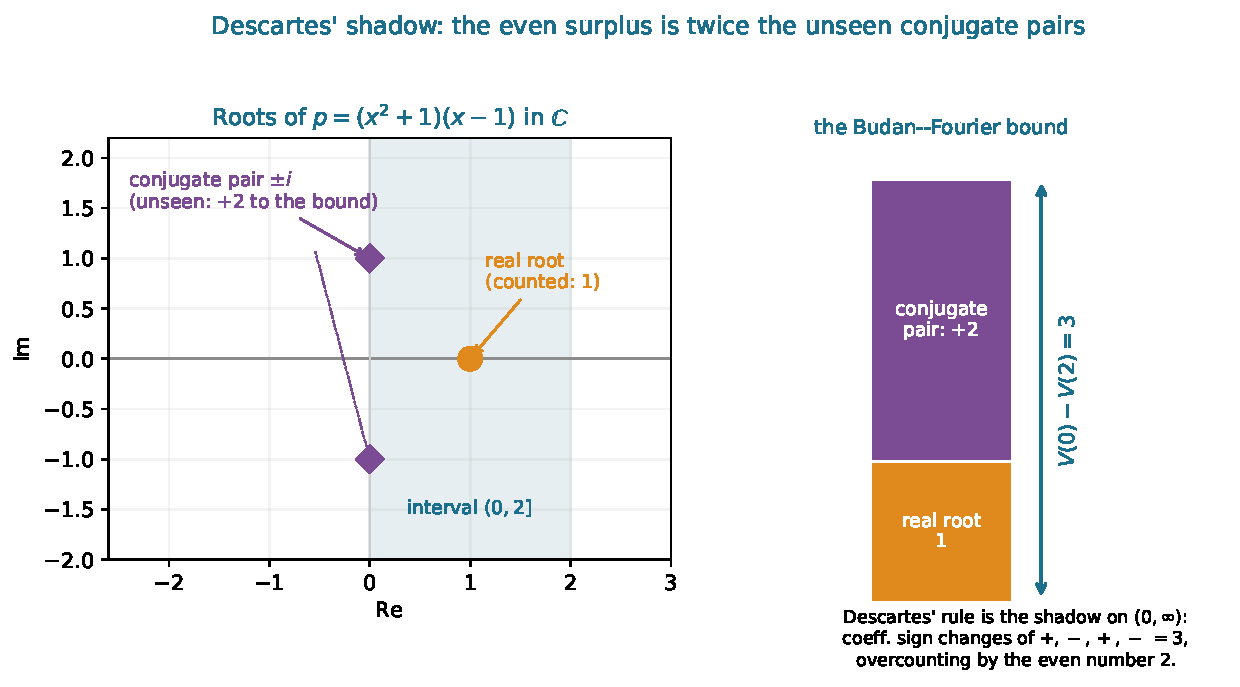
\includegraphics[width=0.88\textwidth]{budan_fig3_shadow}
\caption{La sombra de Descartes. Para $p=(x^2+1)(x-1)$ sobre $(0,2]$ la ca\'ida de la torre es
$\V(0)-\V(2)=3$: la \'unica ra\'iz real $x=1$ aporta $1$, y el par conjugado no visto $\pm i$ aporta el
resto par $2$. Le\'ido sobre $(0,\infty)$ esto es la regla de Descartes---tres cambios de signo de los
coeficientes $+,-,+,-$, sobrecontando la \'unica ra\'iz positiva por un n\'umero par. El excedente es
siempre par porque las ra\'ices complejas de un polinomio real vienen en pares conjugados. Recuentos
afirmados exactamente antes de dibujar.}
\label{fig:shadow}
\end{figure}

\emph{El compa\~nero de Sturm.} Los dos teoremas est\'an ahora uno al lado del otro en el mismo
desarrollo de Lean, sobre un \'unico instrumental de variaci\'on de signo: el recuento exacto de
ra\'ices \emph{distintas} de Sturm sobre la cadena de restos~\cite{sturmlean}, y la cota con
multiplicidad de Budan--Fourier sobre la torre de derivadas. El n\'ucleo compartido---constancia local,
el recuento recursivo de cambios de signo, la recursi\'on del par cabecero---se escribi\'o una vez y se
us\'o dos. Su diferencia es ahora tambi\'en un objeto formal: la cadena de Sturm es coprima y su
an\'alisis local es una sola ca\'ida cabecera; la torre no lo es, y su an\'alisis local es el colapso de
bloque de la Secci\'on~\ref{sec:q2}.

\section{Qu\'e habilita un Budan--Fourier certificado}\label{sec:enables}

M\'as all\'a de Descartes, el teorema certificado es el primer paso verificado del puente cl\'asico al
aislamiento de ra\'ices reales. Un m\'etodo de subdivisi\'on que biseca un intervalo y lee
$\V(a)-\V(b)$ en cada mitad tiene, en este teorema, una garant\'ia verificada por m\'aquina de que el
n\'umero reportado es una cota superior de las ra\'ices y de que cae al recuento verdadero a medida que
los intervalos se encogen en torno a ra\'ices simples; la versi\'on con multiplicidad es exactamente lo
que el aislamiento de ra\'ices m\'ultiples necesita. El desarrollo en Isabelle de Wenda
Li~\cite{liBF} tom\'o esta ruta hacia un procedimiento certificado de recuento de ra\'ices; las piezas
de Lean de aqu\'i son el cimiento sobre el que lo mismo podr\'ia construirse sobre Mathlib. Nada en este
paper construye el aislador---eso se nombra honestamente entre las preguntas abiertas---pero el lema que
soportar\'ia su peso est\'a ya en la biblioteca.

\section{Las piezas}\label{sec:blocks}

La Tabla~\ref{tab:results} re\'une los resultados que soportan el peso, todos \lean{sorry}-free en
\lean{BudanFourier.lean}; la Tabla~\ref{tab:signsB} lee el Ejemplo B sobre su torre, el testigo m\'as
peque\~no del excedente par; la Tabla~\ref{tab:metrics} mide el desarrollo. La dependencia corre como el
mapa del lector (Figura~\ref{fig:readermap}): los dos ladrillos de monoton\'ia alimentan las
recursiones de signo por miembro, que alimentan \lean{signs\_right\_eq\_Rseq}/\lean{signs\_left\_eq\_Lseq};
estas, con las puras \lean{Rseq\_spec}/\lean{Lseq\_spec} y la identificaci\'on de la multiplicidad, dan
la ca\'ida local \lean{fourierVar\_drop\_at\_critical\_point}; y la inducci\'on global sobre los puntos
cr\'iticos ensambla \lean{budan\_fourier}.

\begin{table}[H]
  \centering\footnotesize
  \arrayrulecolor{ggteal}
  \begin{tabular}{@{}llc@{}}
    \toprule
    \rowcolor{ggteal}
    \textcolor{white}{\textbf{Nombre Lean}} & \textcolor{white}{\textbf{Enunciado}} & \textcolor{white}{\textbf{Estado}} \\
    \midrule
    \rowcolor{ggband}
    \lean{budan\_fourier} & $\#\mathrm{ra\acute{\imath}ces}(a,b]\le \V(a){-}\V(b)$ y $\V(a){-}\V(b){-}\#\mathrm{ra\acute{\imath}ces}$ par & probado \\
    \lean{fourierVar\_drop\_at\_critical\_point} & $\exists e,\ \V(a)=\V(b)+\#\mathrm{ra\acute{\imath}ces}(a,b]+2e$ (n\'ucleo local) & probado \\
    \rowcolor{ggband}
    \lean{fourierVar\_eq\_signVarAt} & $\V_p(x)=\lean{signVarAt}\,(\lean{fourierSeq}\,p)\,x$ (puente, \lean{rfl}) & probado \\
    \lean{signs\_right\_eq\_Rseq} & signos en $b$ $=\lean{Rseq}$ de los signos en $c$ (la derecha colapsa) & probado \\
    \rowcolor{ggband}
    \lean{signs\_left\_eq\_Lseq} & signos en $a$ $=\lean{Lseq}$ de los signos en $c$ (la izquierda alterna) & probado \\
    \lean{Rseq\_spec} / \lean{Lseq\_spec} & $\V(c^+){=}\V(c)$;\ $\V(c^-){=}\V(c^+){+}m{+}2g$ (combinatoria) & probado \\
    \rowcolor{ggband}
    \lean{fourierSeq\_isChain} & la torre es una cadena de derivadas $p^{(k+1)}=(p^{(k)})'$ & probado \\
    \lean{sign\_eval\_\{right,left\}\_vanish} & los dos ladrillos de monoton\'ia (signo justo fuera de una ra\'iz) & probado \\
    \bottomrule
  \end{tabular}
  \arrayrulecolor{black}
  \caption{Los resultados que soportan el peso, todos \lean{sorry}-free en \lean{BudanFourier.lean}
  (Lean~4 / Mathlib). \lean{\#print axioms BudanFourier.budan\_fourier} reporta solo \lean{propext},
  \lean{Classical.choice}, \lean{Quot.sound}. Hasta donde s\'e, es la primera formalizaci\'on del
  teorema de Budan--Fourier en Lean.}
  \label{tab:results}
\end{table}

\begin{table}[H]
\centering\small
\rowcolors{2}{ggband!35}{white}
\begin{tabular}{@{}rcccr@{}}
\toprule
\rowcolor{ggteal!18}
$x$ & $p_B=x^2{+}1$ & $p_B'=2x$ & $p_B''=2$ & $\V(x)$ \\
\midrule
$-2$            & $+$ & $-$ & $+$ & $2$ \\
$-1$            & $+$ & $-$ & $+$ & $2$ \\
$0$ {\scriptsize($p_B'{=}0$, no ra\'iz)} & $+$ & $0$ & $+$ & $0$ \\
$1$             & $+$ & $+$ & $+$ & $0$ \\
$2$             & $+$ & $+$ & $+$ & $0$ \\
\bottomrule
\end{tabular}
\caption{Ejemplo B, $p_B=x^2+1$, sin ra\'iz real. $\V$ cae en $2$ en $x=0$---un cero del miembro
interior $p_B'$, \emph{no} una ra\'iz de $p_B$. As\'i $\#\mathrm{ra\acute{\imath}ces}(-2,2]=0<\V(-2)-\V(2)=2$
y el excedente es par: la firma de un par conjugado, y exactamente el caso
\lean{fourierVar\_drop\_at\_critical\_point} con testigo $e=1$.}
\label{tab:signsB}
\end{table}

\begin{table}[H]
  \centering\footnotesize
  \arrayrulecolor{ggteal}
  \begin{tabular}{@{}lr@{}}
    \toprule
    \rowcolor{ggteal}
    \textcolor{white}{\textbf{Cantidad}} & \textcolor{white}{\textbf{Valor}} \\
    \midrule
    \rowcolor{ggband}
    L\'ineas en \lean{BudanFourier.lean} & $940$ \\
    Teoremas / definiciones & $28$ \\
    \rowcolor{ggband}
    \lean{sorry} / \lean{admit} / \lean{native\_decide} & $0$ \\
    Axiomas m\'as all\'a del n\'ucleo de Lean & $0$ \\
    \rowcolor{ggband}
    Reutilizado de \lean{Sturm.lean} & instrumental de variaci\'on de signo \\
    Tiempo de compilaci\'on (Mathlib en caliente) & ${\approx}\,8$\,s \\
    \bottomrule
  \end{tabular}
  \arrayrulecolor{black}
  \caption{El desarrollo, medido. El tiempo de compilaci\'on es para verificar \lean{BudanFourier.lean}
  contra una Mathlib precompilada y la librer\'ia \lean{Sturm} importada, cuyo instrumental de
  variaci\'on de signo se reutiliza.}
  \label{tab:metrics}
\end{table}

\section{La frontera de la contribuci\'on}\label{sec:boundary}

Quiero los l\'imites enunciados sin barniz.

\emph{No es primero en ning\'un sistema.} El teorema de Budan--Fourier se formaliz\'o en Isabelle/HOL
por Wenda Li en 2018--2019~\cite{liBF}, con multiplicidad, y se us\'o all\'i para impulsar un
procedimiento certificado de recuento de ra\'ices; Li tambi\'en extendi\'o una formalizaci\'on previa
del teorema de Sturm en Isabelle para contar con multiplicidad. El presente trabajo es, hasta donde s\'e,
la primera demostraci\'on en \emph{Lean}, basada en b\'usquedas de Loogle y un \lean{grep} de Mathlib en
junio de 2026. El valor es la formalizaci\'on en Lean-y-Mathlib y su maquinaria reutilizable, no la
prioridad sobre Isabelle.

\emph{El cuerpo y la caracter\'istica.} Todo es sobre $\R$. El paso de la multiplicidad usa la
caracter\'istica cero de forma esencial---es lo que hace que el orden de la primera derivada no nula
iguale la multiplicidad de la ra\'iz---as\'i que la demostraci\'on tal como est\'a escrita no se
transfiere tal cual a caracter\'istica positiva, donde esa identidad falla.

\emph{Qu\'e se cuenta y qu\'e no.} El teorema cuenta ra\'ices con multiplicidad y las acota por la
ca\'ida en variaci\'on de signo, con el refinamiento de paridad par. \emph{No} computa las ra\'ices, no
produce un certificado del recuento para una herramienta aguas abajo, y no construye un aislador de
ra\'ices; eso se nombra entre las preguntas abiertas.

\emph{Qu\'e se reutiliza y qu\'e es nuevo.} El instrumental de variaci\'on de signo---constancia local,
\lean{signChanges}, la recursi\'on del par cabecero---se importa del desarrollo de Sturm~\cite{sturmlean}
y no se re-deriva. Nuevos aqu\'i son los dos ladrillos de monoton\'ia, el desacoplamiento
\lean{Rseq}/\lean{Lseq} y sus especificaciones, la identificaci\'on de la racha inicial con la
multiplicidad, y el ensamblaje en la ca\'ida local y el teorema global.

\section{Preguntas reflexivas, para la siguiente cuenta}\label{sec:questions}

Un collar de cuentas est\'a hecho para continuarse. Verificar por m\'aquina un teorema de doscientos
a\~nos no es un fin en s\'i mismo: su valor se mide por lo que las piezas certificadas dejan preguntar a
continuaci\'on, y preguntar con m\'as filo. Cierro con las preguntas que prefiero llevarme antes que
fingir haber resuelto---cada una un lugar donde este trabajo se queda corto, y cada una, creo, no solo
la semilla de otro paper sino un pelda\~no por encima de este.

\begin{enumerate}\itemsep3pt
\item \emph{De cota a certificado.} El teorema dice que la ca\'ida \emph{acota} el recuento y comparte
su paridad; el excedente par mide cu\'anto se pasa la cota. ¿Puede convertirse el excedente en un
\emph{c\'omputo}---un procedimiento verificado que, bisecando hasta que el excedente se anule, devuelva
el recuento exacto con multiplicidad, y un certificado que una herramienta esc\'eptica pueda
reverificar? ¿Cu\'anta de la maquinaria de fracciones continuas de Vincent y
Akritas~\cite{vincent,collinsakritas} querr\'ia el puente honesto?

\item \emph{Portar la unificaci\'on conocida, no atribu\'irsela.} Que los recuentos de Descartes,
Budan--Fourier y Sturm son facetas de un \'unico principio de variaci\'on de signo es cl\'asico, no
m\'io---lo dicen sin rodeos Akritas~\cite{akritas} y Basu--Pollack--Roy~\cite{bpr}---y el invariante
profundo, el \emph{\'indice de Cauchy}, est\'a axiomatizado mediante \emph{cadenas de Sturm} abstractas
por Eisermann~\cite{eisermann} y \emph{ya} se ha verificado por m\'aquina, en Isabelle/HOL, por Li y
Paulson~\cite{liCauchy}. Lo que falta es una formalizaci\'on en \emph{Lean}. Y aqu\'i la torre no es solo
una instancia m\'as: el axioma de cadena de Sturm de Eisermann (su Def.~3.10) exige que cuando un
miembro \emph{interior} se anula, sus vecinos sean estrictamente opuestos, $S_{k-1}\,S_{k+1}<0$---de modo
que no se anulen dos miembros consecutivos a la vez. La torre de derivadas \emph{viola} esto en toda
ra\'iz m\'ultiple, donde $p$ y $p'$ se anulan a la vez; no es una cadena de Sturm en el sentido
cl\'asico. La pregunta abierta honesta es entonces precisa: ¿cu\'al es el axioma m\'as d\'ebil que a\'un
fuerza la ca\'ida local, con el colapso/alternancia de bloque de la Secci\'on~\ref{sec:q2} (los lemas
\lean{Rseq\_spec}/\lean{Lseq\_spec}) como ley local general y la condici\'on antipodal de Eisermann como
su caso especial no degenerado?

\item \emph{Qu\'e es realmente el desacoplamiento.} \lean{Rseq}/\lean{Lseq} separaron la combinatoria de
reescribir una lista de signos del \'algebra que licencia cada reescritura, exactamente como
\lean{FlankReduce} para Sturm. Dos cadenas distintas, la misma forma de argumento: ¿es ``un recuento de
cambios de signo transformado por una reescritura de lista localmente licenciada'' un lema reutilizable
por derecho propio, o simplemente encaj\'o dos veces? Sospecho lo primero y no lo he probado.

\item \emph{El bloque, m\'as all\'a de la caracter\'istica cero y de una variable.} El paso de la
multiplicidad se apoya en la caracter\'istica cero; la torre en s\'i no. ¿Cu\'al es el enunciado correcto
sobre un cuerpo general, donde la racha inicial no tiene por qu\'e igualar la multiplicidad? ¿Y hay un
an\'alogo en base de Bernstein o multivariado del colapso de bloque---el lugar donde el recuento de
ra\'ices en la recta se encuentra con la geometr\'ia de varias variables?
\end{enumerate}

\noindent Lo que une las cuatro es una reflexi\'on. Con el teorema convertido ya en un punto fijo que un
n\'ucleo defender\'a, la direcci\'on interesante ya no es volver a demostrarlo sino preguntar qu\'e puede
sostenerse \emph{sobre} \'el: un certificado, un \'unico principio tras tres recuentos, un patr\'on de
demostraci\'on reutilizable, un cuerpo m\'as amplio. Ninguno meramente extender\'ia el resultado---cada
uno subir\'ia de nivel toda la historia de la torre de derivadas, que es la \'unica clase de
continuaci\'on que merece la pr\'oxima cuenta.

\section*{Reproducir}
\begin{verbatim}
git clone https://github.com/karlesmarin/godsil-gutman-lean
cd godsil-gutman-lean && lake exe cache get
lake build Sturm           # el instrumental de variacion de signo importado
lake env lean BudanFourier.lean
\end{verbatim}
Lean \lean{v4.30.0-rc2}, pin de Mathlib \lean{701fb6e9}. El teorema es
\lean{BudanFourier.budan\_fourier} en \lean{BudanFourier.lean}; sus soportes est\'an en la
Tabla~\ref{tab:results}. \lean{\#print axioms} comprueba que depende solo de \lean{propext},
\lean{Classical.choice}, \lean{Quot.sound}. Los ejemplos trabajados de las Figuras~\ref{fig:tower}
y~\ref{fig:critical} se rederivan, y cada signo y recuento se afirma contra aritm\'etica exacta, antes
de dibujar las figuras (\lean{figures/budan\_fig1\_tower.py}, \lean{figures/budan\_fig2\_critical.py}).

\begin{thebibliography}{99}\small
\bibitem{descartes} R.~Descartes, \emph{La G\'eom\'etrie} (1637); la regla de los signos acota el
n\'umero de ra\'ices positivas por el n\'umero de cambios de signo de los coeficientes.
\bibitem{budan} F.~D.~Budan de Boislaurent, \emph{Nouvelle m\'ethode pour la r\'esolution des
\'equations num\'eriques}, Par\'is (1807; 2\textsuperscript{a} ed.\ 1822).
\bibitem{fourier} J.~Fourier, \emph{Analyse des \'equations d\'etermin\'ees}, Firmin Didot, Par\'is
(p\'ostumo, 1831).
\bibitem{sturm} C.~Sturm, M\'emoire sur la r\'esolution des \'equations num\'eriques, \emph{M\'emoires
pr\'esent\'es par divers savants \`a l'Acad\'emie Royale des Sciences} \textbf{6} (1835) 271--318;
presentado en 1829.
\bibitem{akritas} A.~G.~Akritas, Reflections on a pair of theorems by Budan and Fourier, \emph{Mathematics
Magazine} \textbf{55} (1982) 292--298.
\bibitem{collinsakritas} G.~E.~Collins, A.~G.~Akritas, Polynomial real root isolation using Descartes'
rule of signs, en \emph{Proc.\ SYMSAC~'76}, ACM, 1976, 272--275.
\bibitem{vincent} A.~Alesina, M.~Galuzzi, A new proof of Vincent's theorem, \emph{L'Enseignement
Math\'ematique} \textbf{44} (1998) 219--256.
\bibitem{bpr} S.~Basu, R.~Pollack, M.-F.~Roy, \emph{Algorithms in Real Algebraic Geometry}, 2\textsuperscript{a} ed.,
Algorithms and Computation in Mathematics \textbf{10}, Springer, 2006 (teor\'ia de variaci\'on de signo, Cap.~2).
\bibitem{eisermann} M.~Eisermann, The fundamental theorem of algebra made effective: an elementary
real-algebraic proof via Sturm chains, \emph{Amer.\ Math.\ Monthly} \textbf{119} (2012), no.~9,
715--752; \texttt{arXiv:0808.0097} (``cadenas de Sturm'' abstractas y el \'indice de Cauchy).
\bibitem{liBF} W.~Li, L.~C.~Paulson, Counting polynomial roots in Isabelle/HOL: a formal proof of the
Budan--Fourier theorem, en \emph{Proc.\ 8th ACM SIGPLAN Int.\ Conf.\ on Certified Programs and Proofs
(CPP~2019)}, ACM, 2019, 52--64 (\texttt{doi:10.1145/3293880.3294092}); preprint
\texttt{arXiv:1811.11093}. La entrada del Archive of Formal Proofs ``The Budan--Fourier Theorem and
Counting Real Roots with Multiplicity'' (W.~Li, 2018), \url{https://isa-afp.org/entries/Budan_Fourier.html}.
\bibitem{litarski} W.~Li, L.~C.~Paulson, A formal proof of the Sturm--Tarski theorem, \emph{Archive of
Formal Proofs} (2014), \url{https://isa-afp.org/entries/Sturm_Tarski.html}.
\bibitem{liCauchy} W.~Li, L.~C.~Paulson, Evaluating winding numbers and counting complex roots through
Cauchy indices in Isabelle/HOL, \emph{J.~Automated Reasoning} \textbf{64} (2020), no.~2, 331--360;
\texttt{arXiv:1804.03922}.
\bibitem{eberl} M.~Eberl, Sturm's Theorem, \emph{Archive of Formal Proofs} (2014),
\url{https://isa-afp.org/entries/Sturm_Sequences.html}.
\bibitem{cohen} C.~Cohen, Construction of real algebraic numbers in Coq, en \emph{Interactive Theorem
Proving (ITP 2012)}, LNCS \textbf{7406}, Springer, 2012, 67--82.
\bibitem{mathlib} The mathlib Community, The Lean mathematical library, en \emph{Certified Programs and
Proofs (CPP 2020)}, ACM, 2020, 367--381.
\bibitem{lean4} L.~de Moura, S.~Ullrich, The Lean~4 theorem prover and programming language, en
\emph{Automated Deduction (CADE~28)}, LNCS \textbf{12699}, Springer, 2021, 625--635.
\bibitem{sturmlean} C.~Mar\'in, \emph{The Staircase of Signs: Sturm's Root-Counting Theorem,
Machine-Checked in Lean~4}, Zenodo, 2026, \texttt{doi:10.5281/zenodo.20707348}.
\bibitem{newton} C.~Mar\'in, \emph{The Inward Bow of a Real-Rooted Polynomial: Newton's Inequalities,
Machine-Checked in Lean~4}, Zenodo, 2026, \texttt{doi:10.5281/zenodo.20693064}.
\bibitem{gglean} C.~Mar\'in, \emph{Random Signs into Matchings: A Godsil--Gutman Identity, Formalized
in Lean~4}, Zenodo, 2026, \texttt{doi:10.5281/zenodo.20517350}.
\end{thebibliography}

\end{document}
